
\chapter{Pruebas y evaluación}
\label{pruebas_evaluacion}

\section{Estrategia de pruebas}
\label{sec:estrategia_pruebas}

La estrategia de pruebas y evaluación de EpilexIA se orienta a verificar el comportamiento funcional del sistema, la integración entre sus componentes, el procesamiento y la visualización de señales electroencefalográficas, así como su rendimiento y usabilidad en el contexto de aplicación previsto. Para ello, se consideran procedimientos de verificación técnica y actividades de evaluación con usuarios, con el propósito de obtener evidencias sobre el cumplimiento de los requerimientos establecidos.

Se adopta principalmente un enfoque de pruebas de caja negra, mediante el cual se evalúa el comportamiento observable del sistema a partir de las entradas proporcionadas y las salidas obtenidas, sin requerir el conocimiento de los detalles internos de implementación. Este enfoque permite analizar EpilexIA desde la perspectiva de sus usuarios y de los servicios que ofrece, considerando operaciones como la gestión de pacientes y estudios, la carga de archivos EEG, la visualización de señales, el registro de anomalías, la ejecución del análisis mediante inteligencia artificial y la elaboración de informes médicos.

La estrategia contempla los siguientes ámbitos de evaluación:

\begin{itemize}
    \item \textbf{Pruebas funcionales:} orientadas a comprobar que las funcionalidades del sistema respondan a los requerimientos definidos y produzcan los resultados esperados ante diferentes condiciones de utilización.

    
    \item \textbf{Pruebas de integración:} destinadas a verificar la comunicación y el intercambio de información entre el \textit{frontend}, el \textit{backend}, las bases de datos y los componentes de inteligencia artificial.

    \item \textbf{Pruebas de procesamiento y visualización EEG:} enfocadas en evaluar la carga y representación de señales, la configuración de montajes, filtros y sensibilidad, la navegación temporal y el registro de anomalías. Sus resultados se presentan en los casos PF-05 a PF-09 y en la prueba de integración PI-05.

    \item \textbf{Pruebas de integración con inteligencia artificial:} dirigidas a comprobar la solicitud de análisis, el seguimiento de las ejecuciones y la recuperación y presentación de los resultados generados.

    \item \textbf{Pruebas de rendimiento:} previstas en la estrategia y no ejecutadas en el presente trabajo, destinadas a medir indicadores cuantitativos, como los tiempos de respuesta, la duración de las operaciones, el consumo de recursos computacionales y el comportamiento del sistema bajo diferentes condiciones de carga.

    \item \textbf{Evaluación de usabilidad:} realizada de forma exploratoria y cualitativa, orientada a analizar la eficacia, eficiencia y satisfacción de los usuarios al realizar tareas representativas de su actividad, considerando como referencia los principios establecidos en la norma ISO~9241-11.
\end{itemize}

Para las pruebas funcionales y de integración se utilizaron casos de prueba que especifican la funcionalidad evaluada, el procedimiento de ejecución y el resultado esperado. Las condiciones de cada ejecución y el resultado obtenido se documentan en la sección correspondiente a cada prueba. Esta estructura permitió documentar los comportamientos observados e identificar posibles diferencias respecto de los requerimientos del sistema.

Las pruebas de integración con el servicio de inteligencia artificial y las sesiones con la especialista se ejecutaron sobre la instancia del sistema desplegada en la nube, descrita en la Sección~\ref{subsec:despliegue-nube}.

La evaluación contó con la participación de una médica especialista en epileptología del Hospital Central del Instituto de Previsión Social (IPS), quien accedió a la instancia de EpilexIA desplegada en la infraestructura en la nube de BigQ (Sección~\ref{subsec:despliegue-nube}) desde las instalaciones hospitalarias, utilizando una cuenta individual con el perfil Especialista. Durante su utilización, la profesional comunicó verbalmente observaciones y sugerencias que fueron registradas por el equipo de desarrollo. Estas observaciones dieron lugar a un conjunto de mejoras funcionales, principalmente relacionadas con el visualizador EEG y las herramientas de análisis, que se detallan en el Cuadro~\ref{tab:observaciones-especialista}. Esta actividad se considera una evaluación exploratoria, dado que no incluyó la aplicación de cuestionarios estandarizados ni la medición sistemática de indicadores de usabilidad.

Finalmente, las evidencias obtenidas servirán de base para analizar el cumplimiento de los requerimientos funcionales y no funcionales, así como para valorar los resultados del sistema en relación con los objetivos y la hipótesis planteados en la investigación.

\section{Pruebas funcionales}
\label{sec:pruebas_funcionales}

\begin{nuevotexto}
Las pruebas funcionales verificaron que las operaciones disponibles en EpilexIA respondan a los requerimientos establecidos.
Siguen el flujo de trabajo clínico: la autenticación, el registro de pacientes y estudios, la revisión de las señales, la consulta de los resultados de inteligencia artificial, la elaboración de informes y la auditoría.
Se definieron quince casos, identificados de PF-01 a PF-15, cada uno con su procedimiento y su resultado esperado.
Todos se ejecutaron sobre la interfaz web, con cuentas de los perfiles correspondientes.

El Cuadro~\ref{tab:sintesis_pruebas_funcionales} resume, para cada caso, la verificación realizada y el resultado obtenido.
El procedimiento completo de cada prueba y sus evidencias se presentan en el Anexo~C.

\begingroup
\small
\setlength{\tabcolsep}{4pt}
\renewcommand{\arraystretch}{1.15}
\begin{longtable}{|p{1.25cm}|p{3.4cm}|p{7.6cm}|p{1.75cm}|}
\caption{Resultados de las pruebas funcionales de EpilexIA.}
\label{tab:sintesis_pruebas_funcionales}\\
\hline
\textbf{ID} & \textbf{Funcionalidad} & \textbf{Verificación realizada y resultado observado} & \textbf{Resultado} \\
\hline
\endfirsthead
\multicolumn{4}{c}{\textit{Continuación del Cuadro \thetable}}\\
\hline
\textbf{ID} & \textbf{Funcionalidad} & \textbf{Verificación realizada y resultado observado} & \textbf{Resultado} \\
\hline
\endhead

PF-01 &
Autenticación de usuarios &
Inicio de sesión con credenciales válidas. El sistema presentó el panel de control con las opciones del perfil Especialista. &
Aprobada \\
\hline

PF-02 &
Validación de credenciales &
Inicio de sesión con una contraseña incorrecta. El sistema mostró el mensaje «Credenciales inválidas» e impidió el acceso. &
Aprobada \\
\hline

PF-03 &
Registro de pacientes &
Registro de un paciente ficticio y búsqueda posterior. El paciente quedó disponible para su selección al crear un estudio. &
Aprobada \\
\hline

PF-04 &
Registro de estudios EEG &
Creación de un estudio asociado al paciente, con validación previa del archivo. El estudio figuró en el listado con estado Procesado. &
Aprobada \\
\hline

PF-05 &
Carga de archivos EEG &
Carga de un archivo EDF junto con el estudio. El sistema mostró el progreso de la transferencia y el estado final Procesado. &
Aprobada \\
\hline

PF-06 &
Visualización de señales EEG &
Apertura del estudio en el visualizador. Se presentaron las señales con sus canales y referencias temporales, y la sensibilidad se ajustó entre 100~$\mu$V y 5~$\mu$V. &
Aprobada \\
\hline

PF-07 &
Configuración de montajes &
Cambio entre los montajes Doble Banana y Transversal sobre un mismo intervalo. El sistema actualizó las derivaciones presentadas. &
Aprobada \\
\hline

PF-08 &
Configuración de filtros &
Modificación del corte inferior (1~Hz y 0,5~Hz), del corte superior (70~Hz y 30~Hz) y del filtro de red. La señal se actualizó en cada caso. &
Aprobada \\
\hline

PF-09 &
Registro manual de anomalías &
Marcado de un intervalo de nueve segundos y guardado como anomalía. El registro quedó disponible en el panel de anomalías. &
Aprobada \\
\hline

PF-10 &
Consulta de resultados de IA &
Consulta del panel de anomalías de un estudio analizado: 47 registros, 43 generados mediante IA y 4 manuales, distinguibles por su origen. Desde cada registro se accedió al intervalo correspondiente. &
Aprobada \\
\hline

PF-11 &
Elaboración de informes médicos &
Redacción y guardado de un informe en estado Borrador. El contenido se conservó al volver a consultar el estudio. &
Aprobada \\
\hline

PF-12 &
Restricción de edición de informes &
Consulta del informe de otro especialista. El sistema lo presentó en modo de solo lectura. &
Aprobada \\
\hline

PF-13 &
Cierre de informes médicos &
Cierre de un informe, con confirmación previa. El informe pasó al estado Cerrado y no admitió modificaciones, tampoco después de reiniciar la sesión. &
Aprobada \\
\hline

PF-14 &
Control de acceso según perfil &
Ingreso con cuentas de los tres perfiles. Cada una presentó únicamente las opciones que le corresponden: gestión de usuarios para el Administrador, estudios para el Técnico, y estudios y reportes para el Especialista. &
Aprobada \\
\hline

PF-15 &
Consulta de auditoría &
Consulta del historial de auditoría con filtros por fecha, evento, actor y rol. El sistema presentó los registros correspondientes a cada filtro. &
Aprobada \\
\hline

\end{longtable}
\endgroup

Los quince casos resultaron aprobados: en todos, el comportamiento observado coincidió con el esperado.
Estas pruebas verifican la disponibilidad y el funcionamiento de las operaciones desde la perspectiva de los usuarios.
No evalúan la precisión diagnóstica del modelo ni constituyen una validación integral de la seguridad o del rendimiento, aspectos que se tratan en la Sección~\ref{sec:sintesis-aspectos}.
\end{nuevotexto}

\section{Pruebas de integración}
\label{sec:pruebas_integracion}

\begin{nuevotexto}
Las pruebas de integración verificaron la comunicación entre los componentes del sistema: la interfaz web, el \textit{backend} clínico, las bases de datos, la API de inteligencia artificial y el motor de procesamiento.
A diferencia de las pruebas funcionales, en cada caso se comprobó, además del comportamiento visible en la interfaz, la respuesta de los servicios y el estado almacenado en las bases de datos.

Se definieron diecisiete casos, identificados de PI-01 a PI-17.
Los casos PI-01 a PI-05 corresponden a la autenticación, las sesiones y la persistencia de pacientes y estudios.
Los casos PI-06 a PI-14 corresponden al ciclo de procesamiento mediante inteligencia artificial.
Los casos PI-15 y PI-16 evalúan el comportamiento ante fallos, y el caso PI-17, la sincronización de la información de los informes médicos con el subsistema de IA.

Los casos PI-15 y PI-16 requieren detener servicios de manera deliberada.
Por ello se ejecutaron en un entorno de pruebas local, que replica el despliegue mediante los mismos contenedores, para no afectar la instancia utilizada en el hospital.

El Cuadro~\ref{tab:resumen_pruebas_integracion} resume la verificación realizada y el resultado obtenido en cada caso.
El procedimiento de cada prueba y sus evidencias, que incluyen las respuestas de los servicios y las consultas a las bases de datos, se presentan en el Anexo~C.

\begingroup
\small
\setlength{\tabcolsep}{4pt}
\renewcommand{\arraystretch}{1.15}
\begin{longtable}{|p{1.25cm}|p{3.4cm}|p{7.6cm}|p{1.75cm}|}
\caption{Resultados de las pruebas de integración de EpilexIA.}
\label{tab:resumen_pruebas_integracion}\\
\hline
\textbf{ID} & \textbf{Integración evaluada} & \textbf{Verificación realizada y resultado observado} & \textbf{Resultado} \\
\hline
\endfirsthead
\multicolumn{4}{c}{\textit{Continuación del Cuadro \thetable}}\\
\hline
\textbf{ID} & \textbf{Integración evaluada} & \textbf{Verificación realizada y resultado observado} & \textbf{Resultado} \\
\hline
\endhead

PI-01 &
Autenticación de usuarios &
El inicio de sesión devolvió un \textit{token} JWT, las solicitudes protegidas respondieron con el código HTTP 200 y la sesión quedó registrada en la base de datos. &
Aprobada \\
\hline

PI-02 &
Protección de servicios &
Una solicitud sin \textit{token} recibió el código HTTP 401, sin datos clínicos. El acceso directo al panel de control sin sesión se redirigió al inicio de sesión. &
Aprobada \\
\hline

PI-03 &
Revocación de sesiones &
Después del cierre de sesión, una solicitud con el mismo \textit{token} recibió el código HTTP 401. &
Aprobada \\
\hline

PI-04 &
Persistencia de pacientes &
El paciente registrado desde la interfaz se recuperó, con los mismos datos, mediante una consulta directa a la base de datos. &
Aprobada \\
\hline

PI-05 &
Registro de estudios y archivos EEG &
El estudio, el archivo EDF y sus metadatos (tamaño, duración y frecuencia de muestreo) quedaron almacenados y asociados, y las señales se visualizaron. &
Aprobada \\
\hline

PI-06 &
Creación de ejecuciones de IA &
Cada solicitud de análisis generó una ejecución identificable, registrada en las dos bases de datos. &
Aprobada \\
\hline

PI-07 &
Prevención de ejecuciones duplicadas &
Una nueva solicitud para un estudio con una ejecución activa no generó un trabajo adicional. &
Aprobada \\
\hline

PI-08 &
Recuperación de trabajos pendientes &
El motor tomó los trabajos en cola y actualizó su estado al iniciar el procesamiento. &
Aprobada \\
\hline

PI-09 &
Actualización de actividad del motor &
La señal de actividad del motor se actualizó periódicamente durante el procesamiento. &
Aprobada \\
\hline

PI-10 &
Propagación del estado de ejecución &
Los cambios de estado de la ejecución se reflejaron en la interfaz web. &
Aprobada \\
\hline

PI-11 &
Recuperación de resultados de IA &
Los resultados presentados en la interfaz correspondieron a la ejecución consultada. &
Aprobada \\
\hline

PI-12 &
Inicio automático de ejecuciones &
Los estudios procesados que no contaban con análisis se encolaron de forma automática. &
Aprobada \\
\hline

PI-13 &
Generación de espectrogramas &
El servicio devolvió los datos del espectrograma y la interfaz los presentó. &
Aprobada \\
\hline

PI-14 &
Registro de eventos de IA &
Los eventos del ciclo de ejecución quedaron registrados y pudieron consultarse en la auditoría. &
Aprobada \\
\hline

PI-15 &
Indisponibilidad del servicio de IA &
Con la API de IA detenida durante 49 minutos, el estudio se cargó y se revisó sin generar ejecuciones inconsistentes. Al restablecerse el servicio, el análisis se encoló a los 14 segundos, sin intervención del usuario, y finalizó correctamente. &
Aprobada \\
\hline

PI-16 &
Saturación de la cola de procesamiento &
Con el límite de la cola reducido a 2 y el motor detenido, la solicitud adicional recibió el código HTTP 503 y el mensaje «Cola de análisis IA llena; reintentar más tarde». Al reiniciar el motor, el estudio rechazado se procesó automáticamente. &
Aprobada \\
\hline

PI-17 &
Sincronización de anotaciones médicas &
Las anotaciones manuales y las ventanas confirmadas en los informes se registraron en el subsistema de IA. &
Aprobada \\
\hline

\end{longtable}
\endgroup

Los diecisiete casos resultaron aprobados.
En conjunto, comprueban la integración entre la interfaz web, el \textit{backend} clínico y las bases de datos, y el ciclo completo del subsistema de inteligencia artificial, desde la solicitud del análisis hasta la recuperación de los resultados.
\end{nuevotexto}

\section{Pruebas automatizadas}
\label{sec:pruebas-automatizadas}

\begin{nuevotexto}
Además de las pruebas manuales, cada componente cuenta con una suite de pruebas automatizadas que se ejecuta durante el desarrollo.
El Cuadro~\ref{tab:pruebas-automatizadas} presenta la cantidad de casos de cada suite y el resultado de su ejecución sobre la versión evaluada.

\begin{table}[H]
\centering
\marcanuevo
\caption{Resultados de las pruebas automatizadas por componente.}
\label{tab:pruebas-automatizadas}
\small
\begin{tabular}{|p{3.4cm}|p{6.2cm}|c|c|}
\hline
\textbf{Componente} & \textbf{Herramientas} & \textbf{Casos} & \textbf{Aprobados} \\
\hline
\textit{Backend} clínico & JUnit, Mockito y Spring Security Test & 194 & 194 \\
\hline
\textit{Frontend} & Vitest y Testing Library & 225 & 225 \\
\hline
API de IA & \texttt{unittest} & 55 & 55 \\
\hline
Motor de IA & \texttt{unittest} & 9 & 9 \\
\hline
\textbf{Total} & & \textbf{483} & \textbf{483} \\
\hline
\end{tabular}
\end{table}

Estas pruebas son unitarias y utilizan dependencias simuladas, por lo que complementan a las pruebas de integración pero no las reemplazan.
No se cuenta con pruebas automatizadas de extremo a extremo ni con medición de cobertura de código.
El detalle de las pruebas del \textit{frontend} y de los componentes de inteligencia artificial se presenta en el Anexo~B.
\end{nuevotexto}

\section{Pruebas de integración con el servicio de IA}

Las pruebas de integración con el servicio de
inteligencia artificial tuvieron como propósito
evaluar la comunicación entre el servidor de
aplicaciones de EpilexIA, la API desarrollada
con FastAPI, el motor de procesamiento y la
base de datos especializada en ejecuciones de IA.

Las verificaciones se realizaron en el entorno desplegado de EpilexIA, con los servicios ejecutándose en contenedores Docker.
Se comprobó la disponibilidad del servicio FastAPI mediante solicitudes HTTP, la preparación de las estructuras de persistencia en PostgreSQL y la comunicación entre los servicios.

Sobre este entorno se ejecutó el ciclo completo de procesamiento con seis estudios EEG reales de pacientes del Hospital Central del IPS, cargados en formato EDF tal como los exporta el equipo de adquisición.
Para cada estudio se solicitó el análisis desde la interfaz web y se observó la asignación de un identificador de ejecución, la toma del trabajo por parte del motor, la propagación de los estados hasta la interfaz y, una vez finalizado el procesamiento, la recuperación y presentación de los intervalos identificados en el visualizador EEG.
En los seis casos la ejecución finalizó correctamente.

Todas las ejecuciones se realizaron con el modelo HGB~2.0, descrito en la Sección~\ref{subsec:modelo-vigente-hgb}.
Los resultados fueron revisados por la médica especialista en epileptología, quien clasificó cada intervalo señalado por el modelo y agregó una descripción cuando lo consideró pertinente.
A modo de ejemplo, en uno de los estudios el modelo señaló once intervalos: la especialista confirmó diez como anomalías, identificó el restante como un artefacto de movimiento y registró manualmente una anomalía adicional.
La Figura~\ref{fig:ia-revision-listado} muestra el panel de anomalías de dicho estudio, con las etiquetas y descripciones incorporadas por la especialista.

\begin{figure}[H]
    \centering
    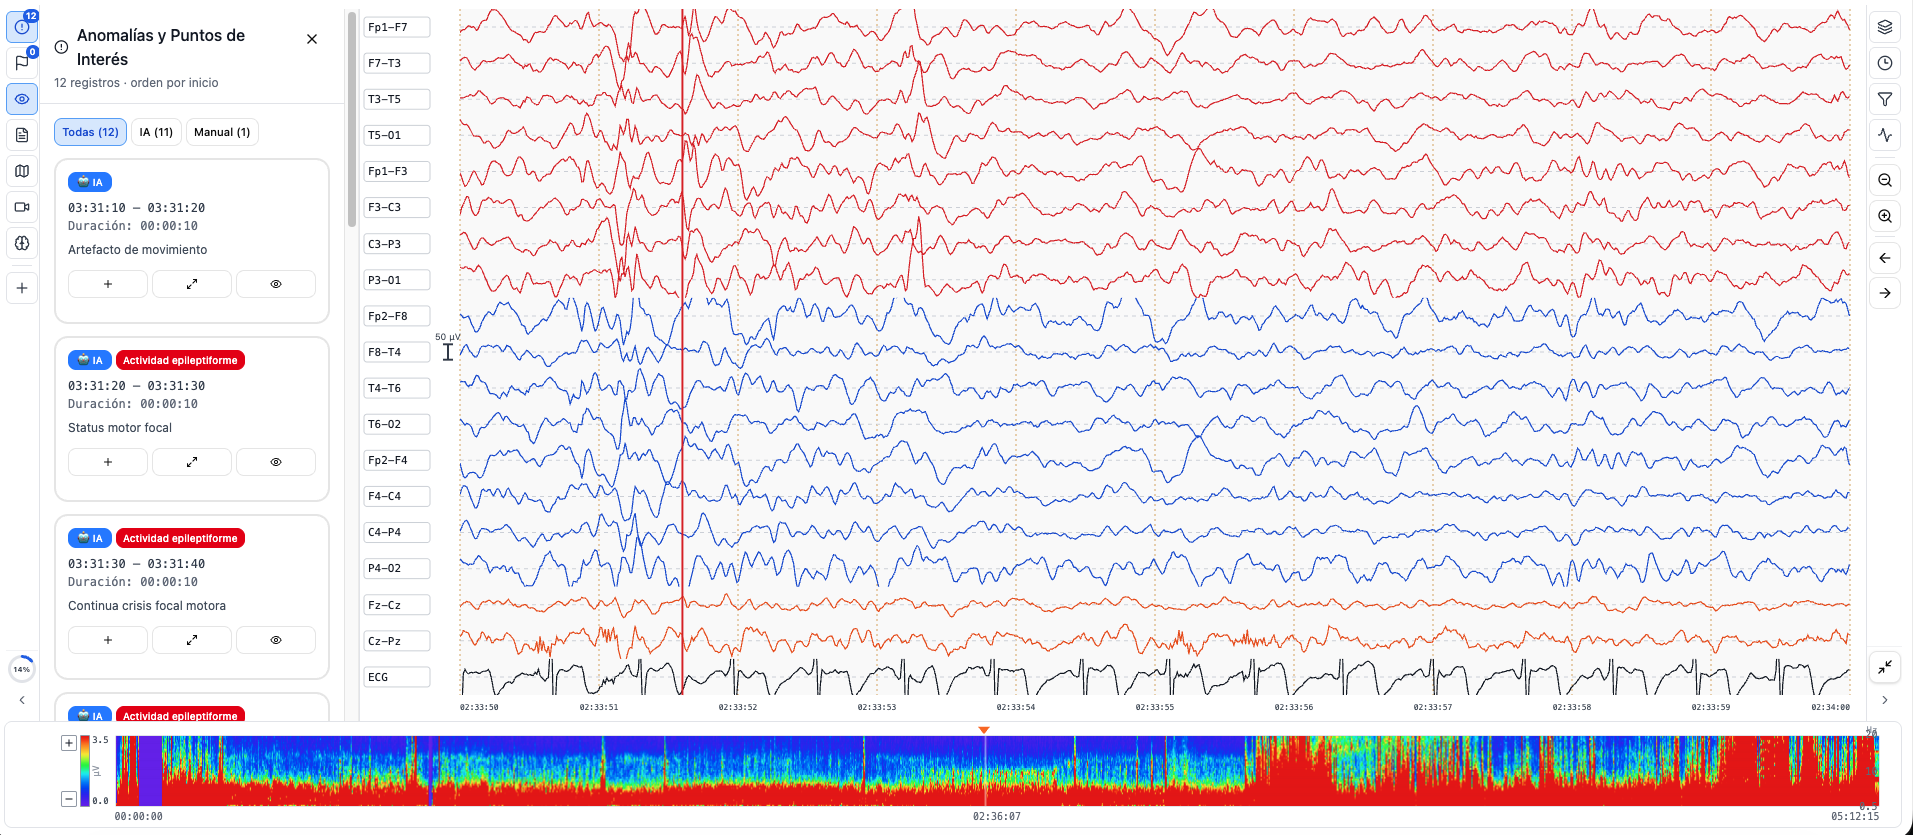
\includegraphics[width=0.95\textwidth]{Chapter6/Chapter6Figs/ia_revision_listado.png}
    \caption{Intervalos identificados por el modelo HGB~2.0 en un estudio real, clasificados y descritos por la especialista en EpilexIA.}
    \label{fig:ia-revision-listado}
\end{figure}

Por consiguiente, las pruebas realizadas permitieron verificar la integración completa entre los componentes del subsistema de IA, desde la solicitud de análisis hasta la presentación de resultados en la interfaz web.
Estas verificaciones corresponden al funcionamiento integrado del sistema sobre un conjunto reducido de estudios y no constituyen una evaluación estadística del desempeño diagnóstico del modelo.

Cabe señalar que la prueba funcional PF-10, descrita anteriormente, se realizó utilizando resultados de inteligencia artificial que ya se encontraban almacenados en la base de datos, por lo que su alcance se limita a la consulta y visualización de dichos registros. La ejecución completa del motor de IA se verificó de manera independiente mediante las pruebas descritas en esta sección.

\section{Evaluación de usabilidad}

La evaluación de usabilidad de EpilexIA incluyó sesiones de prueba con una médica especialista en epileptología del Instituto de Previsión Social (IPS), perteneciente al grupo de usuarios destinatarios de la plataforma. El propósito fue observar la interacción de la profesional con las funcionalidades relacionadas con su actividad clínica.

Durante las sesiones, la especialista realizó tareas representativas del flujo de trabajo previsto, entre ellas la carga de archivos EEG en formato EDF, la exploración de señales electroencefalográficas mediante el visualizador, el marcado manual de posibles anomalías y la elaboración del informe médico correspondiente.

Estas actividades permitieron observar la utilización directa de las herramientas disponibles y comprobar que la profesional pudo completar las tareas descritas en el escenario evaluado.

La evaluación tuvo carácter exploratorio y cualitativo. No se aplicaron cuestionarios estandarizados de usabilidad ni se realizaron mediciones sistemáticas de tiempos de ejecución, tasas de error o satisfacción de la usuaria. Por consiguiente, los resultados no permiten establecer indicadores cuantitativos de eficacia, eficiencia o satisfacción.

La realización de evaluaciones adicionales con un mayor número de profesionales y procedimientos sistemáticos de medición permitiría obtener resultados más representativos sobre la experiencia de uso de EpilexIA.

\section{Validación en el contexto del Hospital Central del IPS}

Como parte de las actividades de validación contextual de EpilexIA, se realizaron sesiones de prueba en el consultorio de una médica especialista en epileptología, ubicado en el Hospital Central del Instituto de Previsión Social (IPS).

Las sesiones se desarrollaron durante los meses de septiembre y octubre de 2026, mediante visitas semanales realizadas los días jueves, de 10:00 a 13:00, con la participación del equipo de desarrollo.
En ellas, la especialista cargó y revisó en la plataforma seis estudios EEG de pacientes del hospital, exportados en formato EDF desde el equipo de adquisición.

La profesional accedió a la plataforma, desplegada en la nube, tanto desde su propia computadora portátil, con el navegador Google Chrome, como desde los equipos del hospital, utilizando en ambos casos sus credenciales de usuario.
En el primer caso empleó su propia conexión a internet y, en el segundo, la red del hospital, lo que permitió observar el comportamiento del sistema con distintos dispositivos y condiciones de conectividad.
Los estudios cargados fueron exportados por la especialista desde el equipo de adquisición del servicio.

Durante las sesiones se desarrolló un flujo de trabajo relacionado con el análisis de estudios electroencefalográficos, cuyas actividades se describieron en la sección anterior. La experiencia proporcionó evidencia inicial de utilización de la plataforma en el contexto institucional para el cual fue concebida.

Durante las sesiones, la especialista formuló observaciones sobre el funcionamiento de la plataforma, que el equipo de desarrollo registró e incorporó de manera progresiva entre una visita y la siguiente.
El Cuadro~\ref{tab:observaciones-especialista} resume dichas observaciones, clasificadas en ajustes de experiencia de uso, corrección de errores y optimizaciones generales del sistema.
Las versiones del sistema descritas en los capítulos anteriores ya incorporan las mejoras implementadas.

\begingroup
\small
\begin{longtable}{|p{0.8cm}|p{9.6cm}|p{2.6cm}|}
\caption{Observaciones surgidas en las sesiones de validación con la especialista y estado de su incorporación.}
\label{tab:observaciones-especialista}\\
\hline
\textbf{N.º} & \textbf{Observación o mejora} & \textbf{Estado} \\
\hline
\endfirsthead

\multicolumn{3}{c}{\textit{Continuación del Cuadro~\thetable}}\\
\hline
\textbf{N.º} & \textbf{Observación o mejora} & \textbf{Estado} \\
\hline
\endhead

\multicolumn{3}{|l|}{\textbf{Ajustes de experiencia de uso}} \\
\hline
1 & Sensibilidad predeterminada de 50~$\mu$V para el canal de ECG. & Implementada \\
\hline
2 & Configuración de filtros independiente para cada canal. & Implementada \\
\hline
3 & Exclusión del canal de ECG de los filtros globales. & Implementada \\
\hline
4 & Incorporación de las derivaciones de línea media del sistema 10-20. & Implementada \\
\hline
5 & Posibilidad de desactivar un canal ante electrodos defectuosos. & Implementada \\
\hline
6 & Colores diferenciados por grupo de derivaciones y para el ECG, de forma análoga al equipo de adquisición. & Implementada \\
\hline
7 & Navegación continua del trazado mediante el teclado y el ratón. & Implementada \\
\hline
8 & Visualización del trazado completo en una única ventana, sin desplazamiento vertical. & Implementada \\
\hline
9 & Espectrograma con referencias temporales para la navegación. & Implementada \\
\hline
10 & Marcado manual de intervalos que se extienden más allá de la ventana visible. & Implementada \\
\hline
11 & Disponibilidad del video en el modo de pantalla completa. & Implementada \\
\hline
12 & Pausa y reanudación del video mediante la barra espaciadora. & Implementada \\
\hline
13 & Ventanas flotantes de tamaño ajustable para el video y el mapa de electrodos. & Implementada \\
\hline
14 & Registro automático en el informe de las anomalías incorporadas, manuales o identificadas mediante IA. & Implementada \\
\hline
15 & Consulta del informe en un panel lateral del modo de pantalla completa. & Implementada \\
\hline
16 & Ejecución del análisis de IA desde el modo de pantalla completa. & Implementada \\
\hline
17 & Avance por ventana con las flechas del teclado y avance continuo por segundo mediante el ratón. & Implementada \\
\hline
18 & Ajuste de la sensibilidad con las flechas del teclado. & Implementada \\
\hline
19 & Sincronización del video al navegar hacia un punto de interés. & Implementada \\
\hline
20 & Ampliación de las etiquetas disponibles para clasificar anomalías. & Pendiente \\
\hline
\multicolumn{3}{|l|}{\textbf{Corrección de errores}} \\
\hline
21 & Corrección de la frecuencia del filtro \textit{Notch} a 50~Hz. & Implementada \\
\hline
22 & Recorte de los trazados al área de su canal, para evitar la superposición con canales adyacentes. & Implementada \\
\hline
23 & Corrección del ordenamiento del listado de anomalías. & Implementada \\
\hline
24 & Unificación del formato de hora (HH:MM:SS). & Implementada \\
\hline
25 & Revisión de la amplitud del canal de ECG con sensibilidad de 50~$\mu$V. & Pendiente \\
\hline
\multicolumn{3}{|l|}{\textbf{Optimizaciones generales del sistema}} \\
\hline
26 & Envío de las anomalías manuales al subsistema de IA para la retroalimentación de los modelos. & Implementada \\
\hline
27 & Optimización del consumo de recursos durante la ejecución del análisis de IA. & Implementada \\
\hline
28 & Procesamiento en paralelo del análisis de IA para estudios pendientes de ejecución. & Implementada \\
\hline
29 & Inicio del análisis de IA una vez finalizadas la carga del estudio y la conversión del video, para evitar la competencia por recursos del servidor. & Implementada \\
\hline
\end{longtable}
\endgroup

No obstante, estas actividades se realizaron con una especialista y no constituyeron una validación clínica integral ni una evaluación estadística del desempeño diagnóstico. La revisión de los resultados del subsistema de inteligencia artificial se efectuó sobre un conjunto reducido de estudios.

En consecuencia, las sesiones aportaron evidencia sobre la utilización de EpilexIA en el entorno hospitalario del IPS. Para determinar su aplicabilidad clínica de manera más amplia, serían necesarias evaluaciones adicionales con otros profesionales y una mayor diversidad de estudios EEG.

Como parte de la preparación para el uso del sistema en el hospital, se elaboraron y entregaron tres documentos: un manual de usuario para los perfiles Especialista y Técnico, un manual para el equipo de TI responsable de la administración del sistema y una guía específica para la exportación y carga de estudios, que es la tarea central del personal técnico.

\section{Síntesis de la evaluación por aspectos de calidad}
\label{sec:sintesis-aspectos}

El Cuadro~\ref{tab:sintesis-aspectos} sintetiza, para cada aspecto de calidad considerado, los puntos cubiertos por las pruebas de este capítulo y por las pruebas automatizadas de los repositorios, y los que no fueron cubiertos.
La organización de la evaluación y de su reporte toma como referencia las guías GEP-HI \citep{Nykanen2011GEPHI} y STARE-HI \citep{Talmon2009STAREHI}.
Las guías y normas citadas se emplean como marco de referencia; el presente trabajo no afirma conformidad ni certificación respecto de ninguna de ellas.

\begingroup
\footnotesize
\setlength{\tabcolsep}{4pt}
\renewcommand{\arraystretch}{1.15}
\begin{longtable}{|>{\raggedright\arraybackslash}p{0.19\textwidth}|>{\raggedright\arraybackslash}p{0.46\textwidth}|>{\raggedright\arraybackslash}p{0.25\textwidth}|}
\caption{Síntesis de la evaluación de EpilexIA por aspectos de calidad.}
\label{tab:sintesis-aspectos}\\
\hline
\textbf{Aspecto y referencia} & \textbf{Puntos cubiertos y pruebas realizadas} & \textbf{Puntos no cubiertos} \\
\hline
\endfirsthead

\multicolumn{3}{c}{\textit{Continuación del Cuadro~\thetable}}\\
\hline
\textbf{Aspecto y referencia} & \textbf{Puntos cubiertos y pruebas realizadas} & \textbf{Puntos no cubiertos} \\
\hline
\endhead

\textbf{Diseño y reporte de la evaluación} \citep{Nykanen2011GEPHI,Talmon2009STAREHI} &
Definición de la estrategia y de los ámbitos de prueba; casos con procedimiento, resultado esperado y resultado obtenido; descripción del contexto, del sistema y de los participantes; declaración de limitaciones. &
Plan formal de evaluación previo a la ejecución; gestión de riesgos del estudio; reporte de la totalidad de los elementos de STARE-HI. \\
\hline

\textbf{Usabilidad} \citep{ISO9241-11:2018,Brooke1996SUS} &
Observación cualitativa, sin medición de indicadores: la especialista completó las tareas del flujo clínico en sesiones semanales durante dos meses. Contexto de uso real: equipos y red del hospital. Observaciones registradas e incorporadas (Cuadro~\ref{tab:observaciones-especialista}). Documentación entregada: manual de usuario para especialistas y técnicos, manual para el equipo de TI a cargo de la administración del sistema y guía específica de carga de estudios. &
Medición de eficacia y eficiencia (tareas completadas, tiempos y errores); satisfacción mediante el cuestionario SUS; más de un participante; perfiles Técnico y Administrador. \\
\hline

\textbf{Rendimiento} &
Sin evaluación. &
Trabajo futuro. \\
\hline

\textbf{Fiabilidad} &
Seguimiento de la actividad del motor (PI-09); comportamiento ante la indisponibilidad del servicio de IA y ante la saturación de la cola, verificado en un entorno de pruebas local (PI-15, PI-16); persistencia de la información tras cerrar y reiniciar la sesión (PF-09, PF-11, PF-13); pruebas automatizadas de los reintentos en la carga de archivos. &
Ensayos de fallos provocados durante el procesamiento. \\
\hline

\textbf{Seguridad y control de acceso} \citep{OWASP2025ASVS} &
Autenticación (PF-01, PF-02, PI-01); gestión y revocación de sesiones (PI-03); autorización por rol y por recurso, verificada también en el \textit{backend} (PF-12, PF-14, PI-02) y mediante pruebas automatizadas; registro de auditoría (PF-15, PI-14). Mecanismos de protección de datos implementados: contraseñas almacenadas mediante \textit{hash}, \textit{tokens} con vencimiento para sesiones y cuentas, enlaces para compartir estudios revocables, enmascarado de datos sensibles en los registros de ejecución, restricciones en la carga de archivos, componentes internos sin exposición a internet y comunicación mediante HTTPS. &
Verificación sistemática frente a los requisitos de la norma; pruebas de intrusión. \\
\hline

\textbf{Privacidad} &
Sin evaluación. &
Trabajo futuro. \\
\hline

\textbf{Fidelidad del visualizador} &
Sensibilidad (PF-06); montajes Doble Banana y Transversal (PF-07); filtros de corte inferior, de corte superior y \textit{Notch} (PF-08); pruebas automatizadas de filtros, unidades, escalas, eje temporal y montajes. &
Comparación cuantitativa con señales de comportamiento conocido. \\
\hline

\textbf{Interoperabilidad} \citep{Kemp1992EDF,KempOlivan2003EDFPlus} &
Lectura de registros EDF y EDF+, con pruebas automatizadas del lector; carga y procesamiento de registros exportados por el equipo de adquisición (PF-05, PI-05); seis estudios reales; conversión del video del equipo de adquisición a MP4; exportación del informe a PDF. &
Importación de las anotaciones de EDF+; comparación con un lector independiente; intercambio con otros sistemas. \\
\hline

\textbf{Accesibilidad} \citep{W3C2023WCAG22} &
Sin evaluación. &
Trabajo futuro. \\
\hline

\textbf{Trazabilidad} &
Auditoría de las acciones por usuario, con consulta y filtros (PF-15); registro de eventos del ciclo de IA (PI-14); identificador, estado y parámetros de cada ejecución (PI-06, PI-10); vínculo entre resultados, ejecución e informe (PI-11, PI-17). &
Reconstrucción documentada de una ejecución completa, del registro EEG al informe. \\
\hline

\textbf{Verificación funcional integrada} &
15 casos funcionales (PF-01 a PF-15) y 17 de integración (PI-01 a PI-17) aprobados; flujo completo sobre seis estudios reales, del registro del estudio al informe; pruebas automatizadas en los repositorios. &
Pruebas automatizadas de extremo a extremo; integración continua; otros navegadores y tamaños de pantalla. \\
\hline

\end{longtable}
\endgroup

Tres aspectos no fueron evaluados y se plantean como trabajo futuro: el rendimiento, la privacidad y la accesibilidad.
Respecto de la privacidad, el subsistema de inteligencia artificial recibe el número de documento del paciente, que se utiliza para vincular los estudios y las ejecuciones entre ambas bases de datos.
Como trabajo futuro se prevé reemplazar el documento por un identificador único sin significado.

\section[Análisis del cumplimiento de los requerimientos]{Análisis del cumplimiento de los \\requerimientos}

El análisis del cumplimiento de los requerimientos
de EpilexIA se realizó considerando las
funcionalidades implementadas y las evidencias
obtenidas durante las pruebas funcionales,
de integración y de utilización del sistema.

Las verificaciones efectuadas permitieron
comprobar el funcionamiento de los mecanismos
de autenticación y autorización, la gestión
de pacientes y estudios electroencefalográficos,
así como el almacenamiento y la visualización
de señales EEG.

Adicionalmente, durante las sesiones de prueba
realizadas con una especialista en epileptología
del IPS, se verificó la utilización de las
funcionalidades de carga de archivos EDF,
marcado manual de posibles anomalías y
elaboración de informes médicos. Esta
experiencia aportó evidencia de uso de
funciones vinculadas directamente con el
trabajo clínico de los profesionales
destinatarios del sistema.

En cuanto al subsistema de inteligencia artificial, se comprobó la disponibilidad de los servicios, la preparación de las estructuras de persistencia y la ejecución integral del procesamiento mediante IA sobre estudios reales, desde la solicitud de análisis hasta la generación, recuperación y presentación de nuevos resultados.

En términos generales, las evidencias obtenidas permiten establecer un cumplimiento verificable de los requerimientos asociados a las funcionalidades de gestión, visualización y procesamiento mediante inteligencia artificial.

Este análisis se limita a los escenarios
efectivamente evaluados y no implica que
todos los requerimientos del sistema hayan
sido comprobados exhaustivamente.

\begin{nuevotexto}
El análisis de estos resultados respecto de los objetivos del trabajo y de la hipótesis planteada se desarrolla en el Capítulo~\ref{chap:conclusiones}.
\end{nuevotexto}
